%xelatex -shell-escape -output-directory=bin ergasia.tex
\documentclass{assignment}

\usepackage{enumerate} % Για την χρησιμοποίηση roman enumerate
\usepackage{paralist} % για το περιβάλλον inparaenum που είναι οι λίστες μέσα στο κείμενο.

\title{Δίκτυα Υπολογιστών \\ 2ο Εργαστήριο: Δυναμική Δρομολόγηση \\ Εργασία: assign2}
\date{Αθήνα, 2015}

\author{Αναγνωστόπουλος Βασίλης - Θάνος (ΜΠΠΛ 13002) \and Βελισσαρίου Κυριάκος (ΜΠΠΛ 13005)}

\begin{document}

\maketitle
% Να σκεφτώ τί αλλαγές θέλω να κάνω με τις αριθμήσεις και άμα θέλω να κάνω.
% Να σκεφτώ να τις ενσωματώσω και στο assignment.cls

\setcounter{page}{1} 
\pagenumbering{roman}

\pagestyle{plain}
\tableofcontents
%\listoftables
%\listoffigures
%\renewcommand\listoflistingscaption{Κατάλογος πηγαίου κώδικα}
%\listoflistings
\newpage

%\pagestyle{headings}
%\pagestyle{fancy}
\setcounter{page}{1} 
\pagenumbering{arabic}


Δίνεται η παρακάτω τοπολογία:

\begin{center}
\resizebox*{\textwidth}{!}{
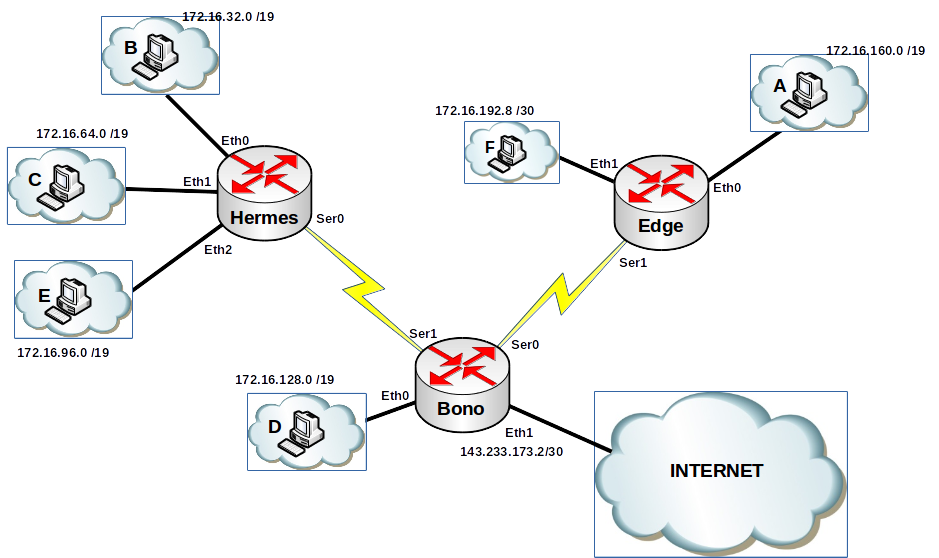
\includegraphics{images/lan.png}}
\end{center}

Ζητούμενα:

\begin{enumerate}

\item Υλοποιήστε την τοπολογία με το λογισμικό που σας δόθηκε. Σε περιπτώσεις όπου δεν δίνονται IP διευθύνσεις, θα πρέπει να υπολογισθούν από εσάς και να αποδοθούν στα αντίστοιχα interface των δρομολογητών. Σημειώστε ότι οι δοθείσες IP διευθύνσεις ανταποκρίνονται στις IP των δικτύων της τοπολογίας – εξαιρείται η διεύθυνση IP του eth1 του δρομολογητή Bono. 

\item Όλοι οι σταθμοί της τοπολογίας πρέπει να έχουν πρόσβαση στην υπηρεσία HTTP που εξυπηρετείται από κάποιον διακομιστή στο Διαδίκτυο. Δεν έχουν πρόσβαση σε κάποια άλλη υπηρεσία του διαδικτύου.

\item Τα δίκτυα που βρίσκονται στον δρομολογητή Hermes είναι προσβάσιμα σε όλους τους άλλους μόνο σε περίπτωση χρήσης των εργαλείων ping και traceroute.

\item Οι δρομολογητές αξιοποιούν τον αλγόριθμο OSPF για τη διαδικασία της δρομολόγησης. 
Προς το Διαδίκτυο χρησιμοποιείται στατική δρομολόγηση.

\end{enumerate}
 
Παραδοτέα:

\begin{enumerate}
  \item Η έκθεση σας:
  \begin{enumerate}
     \item Screenshot της τοπολογίας.
     \item Screenshot που θα εμφανίζει τις επιτυχημένες προσπάθειες πρόσβασης 2 σταθμών στην υπηρεσία HTTP.
     \item Screenshot που θα αποδεικνύει το ζητούμενο 3, όπως διατυπώνεται παραπάνω.
     \item Screenshot με το αποτέλεσμα εκτέλεσης της εντολής \#show ip ospf
     \item Screenshot με το αποτέλεσμα εκτέλεσης της εντολής \#show ip ospf database
  \end{enumerate}
  \item Τα αρχεία (.pkt) με την τοπολογία σας.
\end{enumerate}

\section{Άσκηση 1η}
\subsection*{Εκφώνηση}

Screenshot της τοπολογίας.

\subsection*{Λύση}

\begin{table}
\begin{center}
  \begin{tabular}{|m{2.3cm}|m{2.9cm}|m{3.5cm}|m{3.4cm}|m{3.3cm}|}
    \hline
    Subnet & Subnet Address & Subnet Mask & Host Addresses & BroadCast Address \\ \hline
  SubnetA & 172.16.160.0 & 255.255.224.0 & 172.16.160.1 - 172.16.191.254 & 172.16.191.255 \\ \hline
  SubnetB & 172.16.32.0 & 255.255.224.0 & 172.16.32.1 - 172.16.63.254 & 172.16.63.255 \\ \hline
  SubnetC & 172.16.64.0 & 255.255.224.0 & 172.16.64.1 - 172.16.95.254 & 172.16.95.255 \\ \hline
  SubnetD & 172.16.128.0 & 255.255.224.0 & 172.16.128.1 - 172.16.159.254 & 172.16.159.255 \\ \hline
  SubnetE & 172.16.96.0 & 255.255.224.0 & 172.16.96.1 - 172.16.127.254 & 172.16.127.255 \\ \hline
  SubnetF & 172.16.192.8 & 255.255.255.252 & 172.16.192.9 - 172.16.192.10 & 172.16.192.11 \\ \hline
  SubnetSer1 & 10.1.1.4 & 255.255.255.252 & 10.1.1.5 - 10.1.1.6 & 10.1.1.7 \\ \hline
  SubnetSer2 & 10.1.1.8 & 255.255.255.252 & 10.1.1.9 - 10.1.1.10 & 10.1.1.11 \\ \hline
  SubnetInt & 143.233.173.0 & 255.255.255.252 & 143.233.173.1 - 143.233.173.2 & 143.233.173.3 \\ \hline
  
  \end{tabular}
\caption{Ο πίνακας των υποδικτύων του δικτύου.}
\label{table:VLSM_subnetting}
\end{center}
\end{table}

\begin{table}
\begin{minipage}{\textwidth} 
\begin{center}
  \begin{tabular}{|c|c|c|c|c|}
    \hline
    Device & Interface & IP Address & Subnet Mask & Default Gateway \\ \hline
    \multirow{4}{*}{Hermes} &  Fa8/0 & 172.16.32.1 & 255.255.224.0 & - \\ \cline{2-5}
                            &  Fa7/0 & 172.16.64.1 & 255.255.224.0 & - \\ \cline{2-5}
                            &  Fa6/0 & 172.16.96.1 & 255.255.224.0 & - \\ \cline{2-5}
                            &  Ser5/0 & 10.1.1.5 & 255.255.255.252 & - \\ \hline

    \multirow{4}{*}{Bono}   &  Fa9/0 & 172.16.128.1 & 255.255.224.0 & - \\ \cline{2-5}
                            &  Fa8/0 & 143.233.173.2 & 255.255.255.252 & - \\ \cline{2-5}
                            &  Ser4/0 & 10.1.1.6 & 255.255.255.252 & - \\ \cline{2-5}
                            &  Ser5/0 & 10.1.1.9 & 255.255.255.252 & - \\ \hline

    \multirow{4}{*}{Edge}   &  Fa7/0 & 172.16.160.1 & 255.255.224.0 & - \\ \cline{2-5}
                            &  Fa8/0 & 172.16.192.9 & 255.255.255.252 & - \\ \cline{2-5}
                            &  Ser6/0 & 10.1.1.10 & 255.255.255.252 & - \\  \hline

    PCA & Eth & 172.16.160.2 & 255.255.224.0 & 172.16.191.1 \\ \hline
    PCB & Eth & 172.16.32.2 & 255.255.224.0 & 172.16.32.1 \\ \hline
    PCC & Eth & 172.16.64.2 & 255.255.224.0 & 172.16.64.1 \\ \hline
    PCD & Eth & 172.16.128.2 & 255.255.224.0 & 172.16.128.1 \\ \hline
    PCE & Eth & 172.16.96.2 & 255.255.224.0 & 172.16.96.1 \\ \hline
    PCF & Eth & 172.16.192.10 & 255.255.255.252 & 172.16.192.9 \\ \hline
  \end{tabular}
\caption{Ο πίνακας των ip διευθύνσεων του δικτύου.}
\label{table:VLSM_ip}
\end{center}
\end{minipage}
\end{table}

Η υλοποίηση στο \en{Cisco Packet Tracer} φαίνεται στο σχήμα \ref{fig:cisco}.

\begin{figure}
\begin{center}
\begin{center}
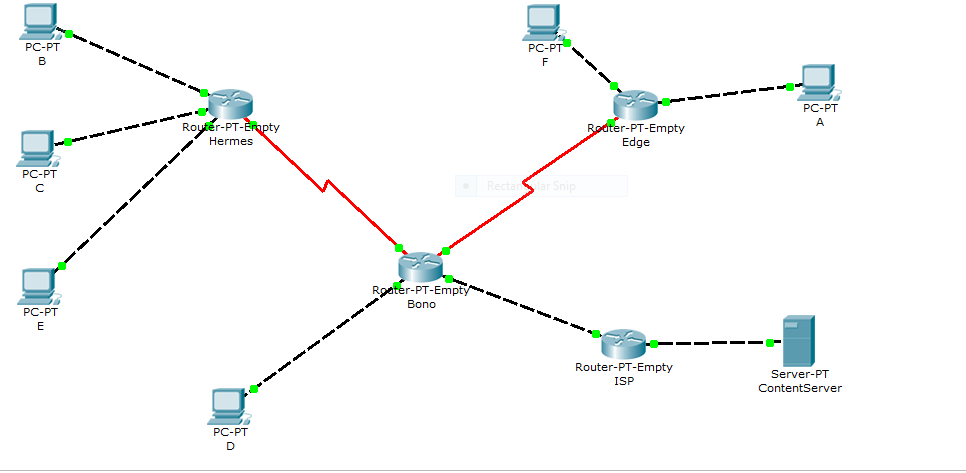
\includegraphics[width=\textwidth, height=\textheight, keepaspectratio]{images/topology.png}
\end{center}
\caption{Η υλοποίηση του δικτύου στο \en{Cisco Packet Tracer}}
\label{fig:cisco}
\end{center}
\end{figure}

\section{Άσκηση 2η}
\subsection*{Εκφώνηση}
Screenshot που θα εμφανίζει τις επιτυχημένες προσπάθειες πρόσβασης 2 σταθμών στην υπηρεσία HTTP.

\subsection*{Λύση}
Για να είναι δυνατή η πρόσβαση των σταθμών στον στην υπηρεσία http και μόνο σε
αυτή, εφαρμόστηκε στο interface Fa8/0 του Bono η εξής ACL:
\captionof{listing}{ACL για το β'}
\begin{minted}[breaklines=true, frame=lines, framesep=2mm, baselinestretch=1.2, fontsize=\footnotesize, linenos]{bash}
permit tcp any any eq www
\end{minted}

Ακολουθούν screenshot από επιτυχημένες προσπάθειες δύο σταθμών στην υπηρεσία
http.
\begin{center}
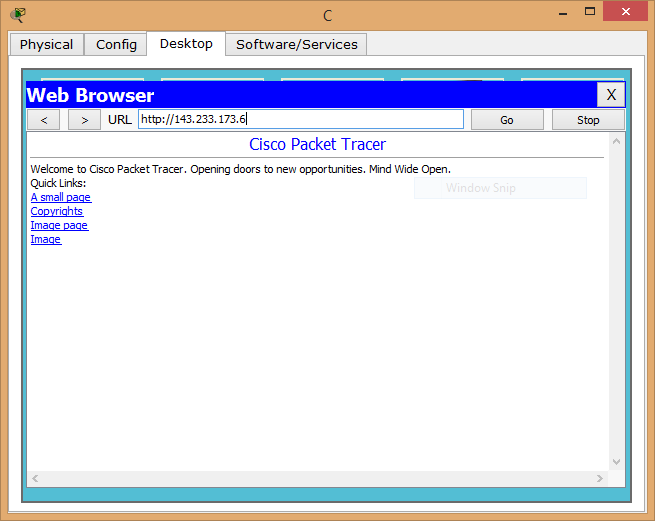
\includegraphics[width=\textwidth, height=\textheight, keepaspectratio]{images/http1.png}
\end{center}

\begin{center}
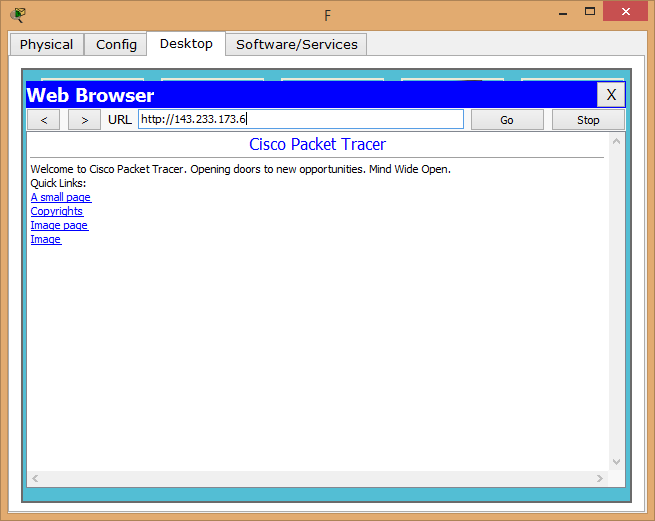
\includegraphics[width=\textwidth, height=\textheight, keepaspectratio]{images/http2.png}
\end{center}

\section{Άσκηση 3η}
\subsection*{Εκφώνηση}

Τα δίκτυα που βρίσκονται στον δρομολογητή Hermes είναι προσβάσιμα σε όλους τους άλλους μόνο σε περίπτωση χρήσης των εργαλείων ping και traceroute.

\subsection*{Λύση}
Σχετικά με το ζητούμενο 3, θέλουμε τα δίκτυα πίσω από τον Hermes να είναι
προσβάσιμα από τους άλλους μόνο για τις υπηρεσίες ping και traceroute. Συνεπώς,
εφαρμόζουμε στα interface Fa6/0, Fa7/0 και Fa8/0 την ACL:

\captionof{listing}{ACL για το γ'}
\begin{minted}[breaklines=true, frame=lines, framesep=2mm, baselinestretch=1.2, fontsize=\footnotesize, linenos]{bash}
permit icmp any any
\end{minted}

Όμως, εάν η ACL έμενε όπως παραπάνω θα υπήρχε το εξής πρόβλημα: Εάν κάποιο
από τα τερματικά πίσω από τον Hermes ήθελε να έχει πρόσβαση στις υπηρεσίες
HTTP του διαδικτύου ναι μεν η αίτηση του θα έφτανε στον ContentServer, αλλά
η απάντηση του Server θα αποριπτόταν από τον δρομολογητή Hermes καθώς επιτρέπει
μόνο εισερχόμενη κυκλοφορία ICMP. Για να λυθεί αυτό το πρόβλημα, και παράλληλα
να ισχύει το ζητούμενο 3, στα παραπάνω interface προστέθηκε και το παρακάτω
φίλτρο στην ACL:
\captionof{listing}{ACL για το γ' (2)}
\begin{minted}[breaklines=true, frame=lines, framesep=2mm, baselinestretch=1.2, fontsize=\footnotesize, linenos]{bash}
permit tcp any any established
\end{minted}
Με το παραπάνω επιτρέπονται τα tcp πακέτα προς τα τερματικά πίσω απο τον Hermes,
αλλά μόνο από επικοινωνία που έχουν ξεκινήσει αυτά τα τερματικά.

Σε ότι αφορά την απόδειξη, στα screenshot της προηγούμενης φαίνεται επιτυχημένο
http request από τερματικό του Hermes. Τέλος, στα δύο screenshot που ακολουθούν
φαίνεται επιτυχημένο ping request προς τερματικό του Hermes, καθώς και
μπλοκαρισμένο πακέτο tcp από επικοινωνία που έχει ξεκινήσει από τερματικό
εκτός του δικτύου Hermes. To τελευταίο επιτεύχθηκε με την λειτουργία simulation
του Packet Tracer.
\begin{center}
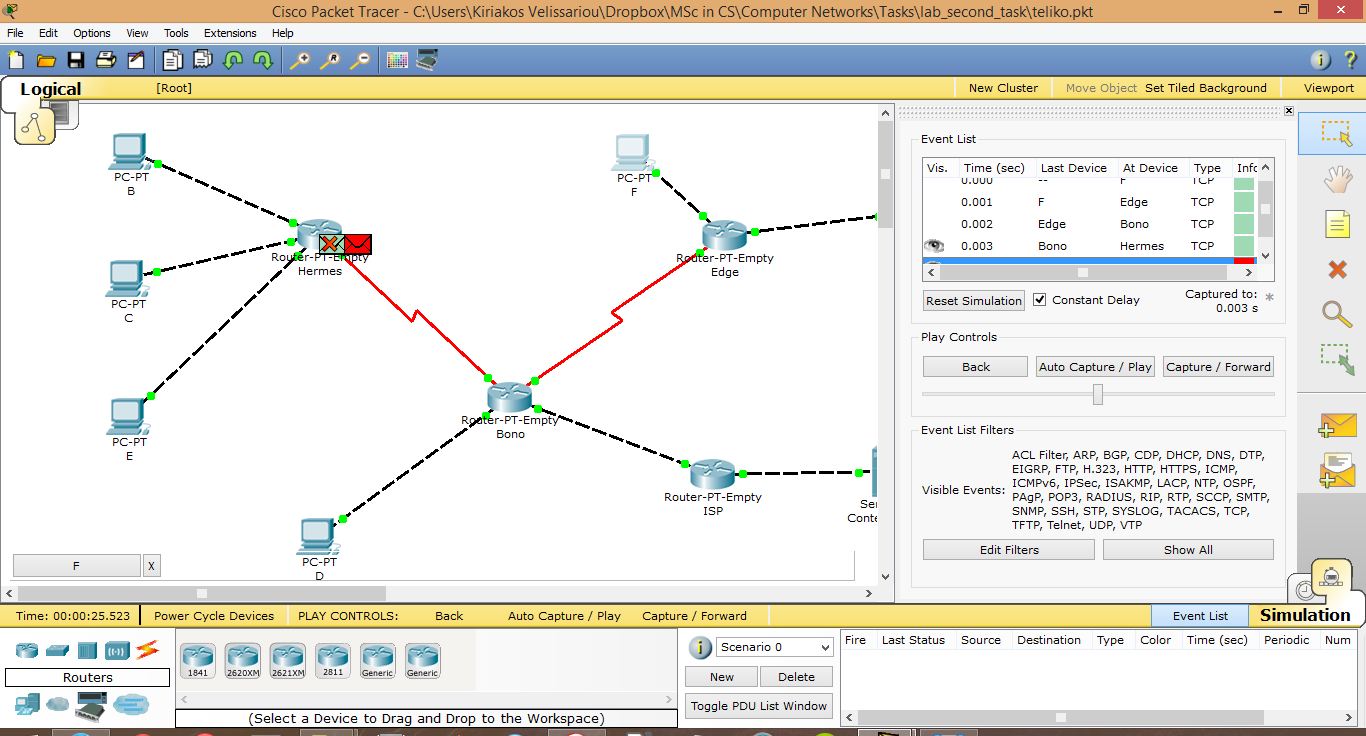
\includegraphics[width=\textwidth, height=\textheight, keepaspectratio]{images/third.png}
\end{center}
\begin{center}
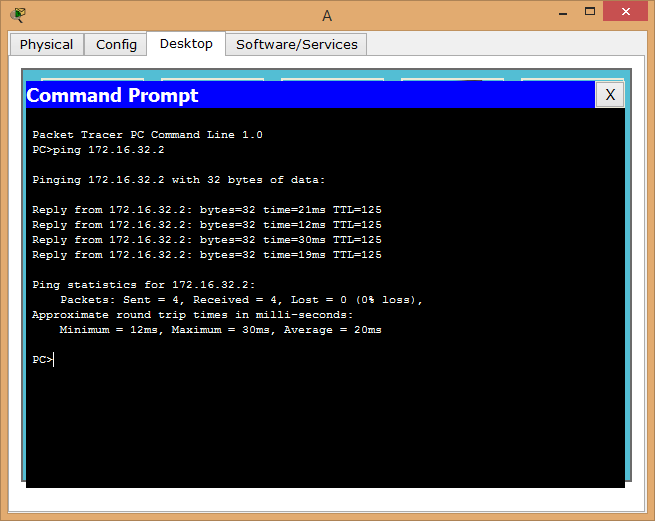
\includegraphics[width=\textwidth, height=\textheight, keepaspectratio]{images/third2.png}
\end{center}

\section{Άσκηση 4η}
\subsection*{Εκφώνηση}

Οι δρομολογητές αξιοποιούν τον αλγόριθμο OSPF για τη διαδικασία της δρομολόγησης. 
Προς το Διαδίκτυο χρησιμοποιείται στατική δρομολόγηση. Εμφάνιση screenshots με
τις εντολές show ip ospf και show ip ospf database.

\subsection*{Λύση}
Σε ότι αφορά το τέταρτο μέρος του παραδοτέου, παρατίθενται screenshots από
τα αποτελέσματα των ζητούμενων εντολών, καθώς και ο κώδικας για την δυναμική
δρομολόγηση.
\captionof{listing}{Οι εντολές για το OSPF στον Hermes}
\begin{minted}[breaklines=true, frame=lines, framesep=2mm, baselinestretch=1.2, fontsize=\footnotesize, linenos]{bash}
Hermes(config)# router ospf 500
Hermes(config-router)# network 172.16.32.0 0.0.31.255 area 0
Hermes(config-router)# network 172.16.64.0 0.0.31.255 area 0
Hermes(config-router)# network 172.16.96.0 0.0.31.255 area 0
Hermes(config-router)# network 10.1.1.4 0.0.0.3 area 0
Hermes(config-router)# ^Z
\end{minted}
\begin{center}
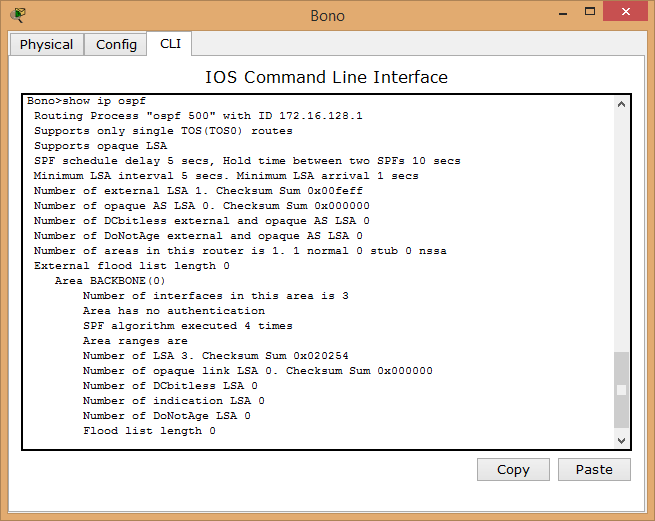
\includegraphics[width=\textwidth, height=\textheight, keepaspectratio]{images/ipsopf.png}
\end{center}

\begin{center}
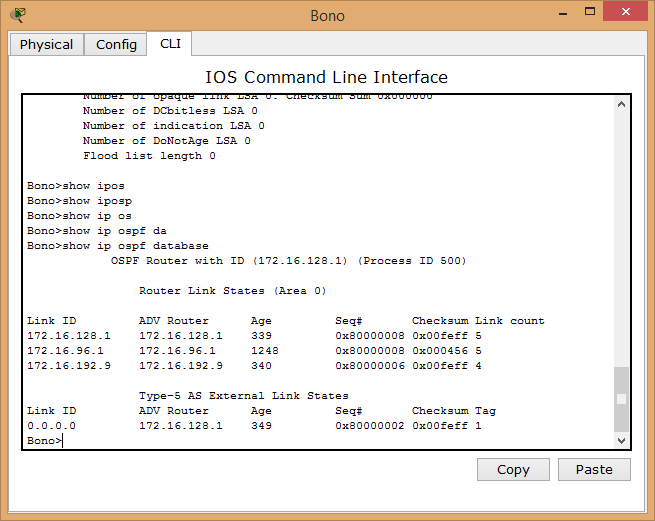
\includegraphics[width=\textwidth, height=\textheight, keepaspectratio]{images/ipospfdb.png}
\end{center}

\captionof{listing}{Οι εντολές για το OSPF στον Edge}
\begin{minted}[breaklines=true, frame=lines, framesep=2mm, baselinestretch=1.2, fontsize=\footnotesize, linenos]{bash}
Edge(config)# router ospf 500
Edge(config-router)# network 172.16.192.8 0.0.0.3 area 0
Edge(config-router)# network 172.16.160.0 0.0.31.255 area 0
Edge(config-router)# network 10.1.1.8 0.0.0.3 area 0
Edge(config-router)# ^Z
\end{minted}

\captionof{listing}{Οι εντολές για το OSPF στον Bono}
\begin{minted}[breaklines=true, frame=lines, framesep=2mm, baselinestretch=1.2, fontsize=\footnotesize, linenos]{bash}
Bono(config)# router ospf 500
Bono(config-router)# network 172.16.128.0 0.0.31.255 area 0
Bono(config-router)# network 10.1.1.8 0.0.0.3 area 0
Bono(config-router)# network 10.1.1.4 0.0.0.3 area 0
Bono(config-router)# ^Z
\end{minted}

\section{Διευκρινήσεις}
Για την προσομοίωση του διαδικτύου χρησιμοποιήθηκε ένας isp δρομολογητής
και ένας εξυπηρετητής. Επίσης, εφαρμόστηκε overloaded NAT έτσι ώστε όλες οι ιδιωτικές
διευθύνσεις να μεταφράζονται στην δημόσια διεύθυνση που αντιστοιχεί στο
interface Fa8/0 του δρομολογητή Bono πριν βγουν προς το διαδίκτυο. Αυτό επετεύχθη με την χρήση της ip access list NAT. Τέλος, ορίστηκε σαν default διαδρομή
το interface Fa8/0 του Bono.
%\phantomsection \label{Βιβλιογραφία}
%\addcontentsline{toc}{section}{Βιβλιογραφία}
%\mtcaddchapter[Βιβλιογραφία] % Λόγω του minitoc
%\bibliographystyle{plain}
%\bibliography{references}

\newpage

\end{document}

